\documentclass[10pt,twoside,slovak,a4paper]{article}

\usepackage[slovak]{babel}
\usepackage[IL2]{fontenc}
\usepackage[utf8]{inputenc}
\usepackage{graphicx}
\usepackage{url} 
\usepackage{hyperref} 

\usepackage{cite}



\title{Gamifikácia a seriózne hry v medicínskom vzdelávaní\thanks{Semestrálny projekt v predmete Metódy inžinierskej práce, ak. rok 2022/23, vedenie: Ing. Ladislav Zemko}}

\author{Petra Miková\\[2pt]
	{\small Slovenská technická univerzita v Bratislave}\\
	{\small Fakulta informatiky a informačných technológií}\\
	{\small \texttt{xmikova@stuba.sk}}
	}

\date{\small 6. november 2022}



\begin{document}

\maketitle

\begin{abstract}
Celosvetovo sa vo veľkom množstve zvyšuje počet pacientov rôznych ochorení, čo v konečnom dôsledku vyžaduje vyšší počet medicínsky vzdelaných ľudí a zvyšuje aj nárok na ich kompetenciu. Veľkým problémom je však nedostatok možností na praktickú výučbu a zastaralé metódy memorovania častí ľudského tela. Aj v tomto smere dokáže pomôcť informatika a jej odvetvia, a preto by som sa v tomto článku primárne chcela venovať využitiu gamifikácie na motiváciu študentov medicíny k učeniu sa a serióznych hier, najmä využívajúcich virtuálnu realitu, na nadobúdanie skúsenosti v oblasti operačných úkonov. Mojim cieľom je v článku ukázať, ako spomínané prostriedky dokážu zefektívniť medicínske vzdelávanie a pomáhať tak riešiť globálny problém.
\ldots
\end{abstract}



\section{Úvod}

Vo svete už od pradávna ľudstvo potrebovalo lekárov, v minulosti skôr ľudí označovaných ako liečiteľov, až pokým nebol zavedený termín lekár. Rozdiel medzi dnešnými lekármi a liečiteľmi pred pár stovkami rokov je však ten, že v dnešnej dobe lekár svoje poznatky nemusí nadobúdať formou pozorovania a skúšania rôznych liečiv a prístupov k ochoreniam \footnote{V súčasnosti stále prebieha výskum ochorení a nových foriem liečby, v našom prípade však hovoríme o nám známych ochoreniach a diagnózach, ktorých liečba už je stanovená a je dokázaná jej efektivita.}, ale vie tieto poznatky nadobudnúť z už publikovaných odborných učebníc a materiálov. Ako však vieme, klasické memorovanie textu v učebniciach sa ukázalo ako neefektívne \cite{Klemm2007WhatGI} nie len pre budúcich lekárov, ale aj všetkých študentov, čomu sa bližšie budeme venovať v časti ~\ref{prvacast}. V časti ~\ref{prvacast} sa taktiež budeme venovať aj problému s nedostatkom možností a materiálov na praktickú výučbu medikov, ktorá predstavuje kľúčovú úlohu v medicínskom vzdelávaní. V tomto článku sa teda budeme sústrediť na dve technologické vymoženosti zefektívňovania vzdelávania medikov – gamifikáciu a seriózne hry, ktorým sa budeme podrobnejšie venovať v častiach ~\ref{druhacast} a ~\ref{tretiacast}. V závere ~\ref{zaver} si zhrnieme našu tému a dôjdeme k zhodnoteniu využitia spomínaných technológii v oblasti medicínskeho vzdelávania.



\section{Hlavný problém} \label{prvacast}
V tejto časti si priblížime hlavný problém, ktorým je zaužívané neefektívne memorovanie učiva z odborných medicínskych učebníc a nedostatočná praktická výučba medikov v dnešnej dobe. 

\subsection{Nadobúdanie poznatkov neefektívnou formou} \label{prvacast:sub1} 
Na každého študenta medicíny sú kladené vysoké nároky čo sa týka množstva vedomostí. Keďže štúdium medicíny je zväčša o memorovaní kvanta informácii o ľudskom tele, je dôležité k nemu pristupovať efektívnym spôsobom, aby študent vedel tieto poznatky využiť aj v praxi a pamatäl si ich čo najdlhšie. Študenti sa všeobecne často potýkajú s javom, že po skúške dané učivo z veľkej časti do pár dní zabudnú \cite{JimmyLIforget}. To je veľmi často práve faktom, že pristupujú k učeniu neefektívne a informácie prijímajú len na krátky čas. Pri medikoch je tento jav však veľmi nebezpečný, pretože ovládať poznatky zo štúdia je kľúčové pri pristupovaní k liečbe pacientov.

\subsection{Problémy s praktickou výučbou} \label{prvacast:sub2} 
Ako už bolo spomenuté v úvode, dôležitou súčasťou medicínskeho vzdelávania je aj praktická výučba. Je samozrejmé, že na vykonávanie lekárskych úkonov nepostačuje len teoretický základ vedomostí, ale hlavne je potrebná už spomínana prax. Taktiež je však dôležitá aj vizualizácia pri učení anatómie ľudského tela a možnosť si časti tela chytiť do rúk a vidieť ich v realite z viacerých uhlov a nie len z ilustrácií v učebniciach, čo dodáva na kompetencii a úrovni vzdelania budúcich lekárov. Problémom však je, že pri praktickej výučbe je počet kadávrov\footnote{mŕtve telá určené práve na výučbu medicíny} obmezdený a každý študent sa ku kadávru dostane na nedostatočný čas. Študenti medicíny potrebujú pozorovať a skúmať tvar kadávru, aby vedeli pochopiť funkciu anatomických štruktúr a identifikovať miesto možného ochorenia. Avšak aj samotný kadáver má svoje mínusy - samozrejme nereaguje na pohyb a farby a štruktúry orgánov sa môžu líšiť od reálnych.\cite{9611852}

\paragraph{}
Je preto veľmi dôležité využit možnosti informatiky a študentom medicíny poskytnúť digitálne média na štúdium ľudského tela. Práve gamifikácia vie dopomôcť k efektívnemu memorovaniu učiva pomocou rôznych foriem odmien a prvkov hier v aplikácii na učenie a virtuálna realita vie pomôcť pri vizualizácii ľudského tela, ako aj pri výučbe operácii a iných úkonov.



\section{Gamifikácia v medicínskom vzdelávaní} \label{druhacast}
Ako už bolo spomenuté, gamifikácia využíva aplikáciu hernej mechaniky, estetiky a herného myslenia na motiváciu k činnosti, v tomto prípade na motiváciu k učeniu sa medicíny. V mobilnej či desktopovej aplikácii sú použité prvky ako skóre, odznaky za splnené ciele, či časové obmedzenia na naučenie sa daného učiva, ktoré prispievajú k efektívnemu sa učeniu. \cite{RojasGamification} Ďalšou možnostou je odosielanie notifikácii po určitom čase od prvého naučenia sa nejakej témy, čo u študentov vyvolá tzv. "spaced repetition", ktorá predstavuje formu efektívneho memorovania. Dôležitú rolu zohráva aj bodovací systém, vďaka ktorému študenti vedia priebežne sledovať svoj pokrok, a taktiež je vďaka tomu možné zostaviť rebríček, kde sa medici vedia porovnať so svojimi rovesníkmi. Motiváciou pre študenta vie byť aj fakt, ak je oproti ostatným medikom s učivom pozadu, čo prirodzene vyvolá snahu o zlepšenie a dorovnanie sa ostatným. \cite{RojasGamification}

\subsection{Návrh aplikácie s využitím gamifikácie pre štúdium medicíny} \label{druhacast:aplikacia} 
Je mnoho prístupov, akými sa dá vytvoriť vzdelávacia aplikácia pre medikov za pomoci gamifikácie. V tejto časti predstavím vlastný návrh, v ktorom vychádzam sčasti z už prezentovaného návrhu z publikácie \cite{9611852}. Pri otvorení uživateľ, v mojom prípade medik, vidí jemu prístupné levely, ktoré si odomýka neskôr práve zbieraním bodov v testoch z predošlých levelov. V každom leveli je sprístupnený materiál s 3D vizualizáciou a prichystané testy, keď sa medik cíti dostatočne pripravený ich absolvovať. Po prvom pretestovaní, ktoré ešte nie je priamo bodovo hodnotené, mu je sprístupnený materiál sústreďujúci sa práve na učivo v ktorom počas pretestovania medik urobil chybu. Po čase z aplikácie dôjde notifikácia k opätovnému zopakovaniu materiálu, aby sa učivo medikovi upevnilo. Na konci každého levelu je finálny test, kde medik získa body, a je len na ňom, aby tieto body postačovali na odomknutie ďalšieho levelu s učivom. Z bodov je možné vytvoriť aj rebríček, kde by sa medik vedel porovnať s rovesníkmi, aj keď neskôr v prieskume ukážem, že porovnávanie sa nemá až taký vplyv na motiváciu k učeniu.


\begin{figure*}[tbh]
\centering
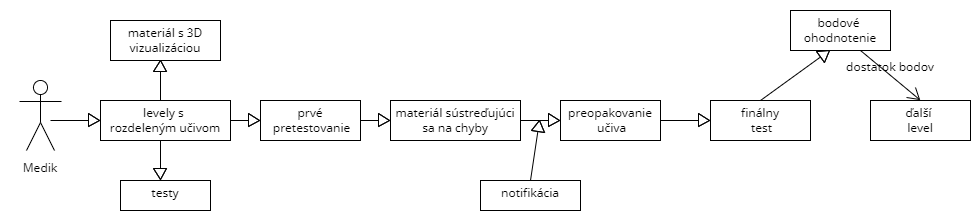
\includegraphics[scale=0.35]{dia.png}
\caption{Diagram zobrazujúci funkcionality aplikácie pre učenie medikov.}
\label{diagram}
\end{figure*}






\section{Prax medikov a využitie serióznych hier} \label{tretiacast}
V časti ~\ref{prvacast} sme si priblížili spôsob praktickej výučby medicíny, ktorá prebieha najmä na kadávroch, aj keď v neskoršom štádiu štúdia sa medici učia vykonávať operačné úkony na reálnych pacientoch. Kadávrov je však vo všeobecnosti nedostatok, a preto je efektívnejšie pristúpiť na výučbu, najmä anatómie, pomocou virtuálnej reality. Virtuálna realita nám v tomto prípade umožňuje využívať 3D priestor na pochopenie priestorových vzťahov medzi časťami tela. S týmito časťami je možné interagovať a manipulovať práve v prostredí virtuálnej reality za pomoci dostupných periférií.  \cite{9678721}
%doplniť časť o menšom riziku vyučby operacii s vyuzitim VR, seriozne hry na surgery training



\section{Reakcia na témy z prednášok} \label{prednasky}


\section{Záver} \label{zaver} 



\bibliography{literatura}
\bibliographystyle{plain}
\end{document}
